\documentclass{edm_template}
\usepackage{amsmath}
%\usepackage[inline]{trackchanges}
\usepackage{natbib}
\usepackage{multirow}
\usepackage[table,usenames]{xcolor}
\definecolor{hcolor}{rgb}{0.5,0,0.25}
%\usepackage[pdftex,pdfborder={0 0 0},colorlinks=true,allcolors=darkblue]{hyperref}
\usepackage[pdftex,pdfborder={0 0 0},colorlinks=true,allcolors=hcolor]{hyperref}
\usepackage{booktabs}
\usepackage{paralist}
\usepackage[utf8]{inputenc}
\usepackage{soulutf8}
\usepackage{graphicx}
\usepackage{rotating}
\usepackage{soul}
\usepackage{flushend}
%\pdfpageheight=11in
%\pdfpagewidth=8.5in
%\usepackage[letterpaper]{geometry}

\DeclareMathOperator*{\argmax}{argmax} % thin space, limits underneath in displays

\newcommand{\dalite}{DALITE}

\begin{document}
% Copyright
%\setcopyright{acmcopyright}
%\setcopyright{acmlicensed}
%\setcopyright{rightsretained}
%\setcopyright{usgov}
%\setcopyright{usgovmixed}
%\setcopyright{cagov}
%\setcopyright{cagovmixed}

% ISBN
\isbn{}

%\conferenceinfo{EDM 2019}{Montreal, Canada}

\newcommand{\Mem}[1]{\hl{[#1]}}
\newcommand{\Mmathsym}[1]{\mathrm{#1}}

\title{Filtering non-relevant short answers in peer learning applications}

\numberofauthors{4}

\newcommand{\ignore}[1]{}
\author{
% 1st. author
\alignauthor
Vincent Gagnon\\
    \affaddr{Polytechnique Montr\'{e}al}\\~\\
% 2nd. author
\alignauthor
Audrey Labrie\\
    \affaddr{Polytechnique Montr\'{e}al}\\
\and
\alignauthor
Sameer Bhatnagar\\
    \affaddr{Polytechnique Montr\'{e}al}\\
\alignauthor
Michel C. Desmarais\\
    \affaddr{Polytechnique Montr\'{e}al}\\
}
\ignore{
% 1st. author
\alignauthor
1st. author\\
    \affaddr{Institution}\\~\\
% 2nd. author
\alignauthor
2nd. author\\
    \affaddr{Institution}\\
\and
\alignauthor
3rd. author\\
    \affaddr{Institution}\\
\alignauthor
4th. author\\
    \affaddr{Institution}\\
}

\maketitle


\begin{abstract}
Applications that adopt peer instruction and active learning make use of short student answers as a learning opportunity: they take some answers as topics of discussion in class, or select answer rationales from peers to foster self-reflection on the learner's own rationale to a question.  However, experience with these applications reveals that some answers are irrelevant, inappropriate, or could even be offensive, and must therefore be filtered out.  Automatic identification of these rationales is the topic of this research.  We introduce an easy-to-implement approach based on standard text classification techniques, namely bag of words and vector space models, and show its effectiveness for filtering irrelevant answers.
\end{abstract}

\keywords{Student response systems, Short answer grading, Vector space model}

%%%%%%%%%%%%%%%%%%
\section{Introduction}

Contemporary student response systems (SRS)~\cite{kaleta2007student,farris2017using} allow students to provide free-text answers to short open-ended questions.  These open-ended questions better enable teachers to capture student's higher level of understanding than close-ended questions~\cite{reilly2014scoring}.  Answers to open-ended questions can serve for in-class discussion and feedback, such as in Socrative~\cite{nawalaniec2015socrative}.  They also serve in out-of-class peer-instruction, as in \dalite~\cite{bhatnagar2016dalite} where other student's answer rationals are presented to students to nurture self-reflexion on a student's own rational.  

However, experience with SRS shows that a small proportion of the answers given by students are inappropriate and should not be presented to their peers.  Filtering out these answers by reading through them is a daunting task.  For example, with over 100k answer rationals currently in our own system, \dalite, the task is highly demanding.  With answers that are shown in-class, as with Socrative, pre-screening would take up too much teacher attention and would not scale well to large classes.  An automatic means to filter unwanted answers is therefore paramount to such SRS.  The goal is to identify student answers that are deemed irrelevant or inadequate for in-class discussion or for inducing student self-reflection on the topic.

This problem is similar to spam-filtering to the extent that it is a binary classification to filter undesired answers, but it also draws from the problem of automatic short answer grading to the extent that desired answers are related to a topic and to a specific question.  While the topic of automatic short answer grading dates back to the 1960's and is still an active field of research (see~\cite{galhardi2018machine,mcdonald2017short,sultan2016fast} for some recent advances), we propose an approach to filter unwanted student answers that relies on a simple Bag of Words (BOW) method to classify undesired answers from relevant ones.

%%%%%%%%%%%%%%%%%%%%%%%%%%%%%%%%%%%%%%%%%%%%%%%%%%%%%%%%%%%%%%%%%%%%%%%%%%%%%
\section{Proposed filtering method}

Building on the idea that a binary relevant/non-relevant classification is the goal and on the principle that correct answers will dwell on a specific topic, the proposed method rests on the principle that irrelevant student answers will contain words that are unrelated to the ones of the relevant answers.  In that respect, an irrelevant answer is expected to be close to orthogonal to all other answers in a vector space model~\cite{turney2010frequency}.

Examples of non-relevant answers are, for eg.:

\begin{tabular}{|l|}
\hline
\textit{Books for sale}\tabularnewline
\textit{idk} (for ``I do not know'')\tabularnewline
\textit{I think thats what it is because i am guessing}\tabularnewline
\textit{Who knows, man. It's gotta be constant}\tabularnewline
\textit{four more years!}\tabularnewline
\textit{.}\tabularnewline
\textit{a} (for choice a)\tabularnewline
\hline
\end{tabular}

As can be seen, answers are often very short, but not always. They are sometimes humorous or sarcastic, or simply expressions of frustrations or disengagement.  But they are characterized by a vocabulary that is unrelated with the questions domain: physics and ergonomics in our two corpuses. Yet, the vocabulary used is generally non-specific to the domain of the question, which is the assumption behind the proposed approach.

To measure the general orthogonality of an answer, we average the cosine of each answer with all other answers.  Given a document-term matrix of~$n$ student answers (documents) by~$t$ terms, $\mathbf{A}_{n \times t}$, the average cosine of answers~$d_i$ in corpus~$D$ is defined as:
\[ \overline{\textrm{cos}}_D(d_i) = \frac{\sum_{j \in D} |\textrm{cos}(d_i, d_j)|}{|D|} \]
where $|D|$ is the corpus size and~$|\textrm{cos}(d_i, d_j)|$ is the absolute value of the cosine between answers~$d_i$ and~$d_j$.

To create the term-document matrix, $\mathbf{A}_{n \times t}$, we apply the common practice of word stemming and spell correction.  The \texttt{tm}\footnote{\url{https://cran.r-project.org/web/packages/tm/tm.pdf}} package is used for this purpose~\cite{nemeth2011hunspello}. The term-document matrix is also transformed using the standard TF-IDF calculated from the corpus.  


%%%%%%%%%%%%%%%%%%%%%%%%%%%%%%%%%%%%%%%%%%%%%%%%%%%%%%%%%%%%%%%%%%%%%%%%%%%%%
\subsection{Answer relevance classification}

The next step is to use the average cosine, $\overline{\textrm{cos}}_D(d_i)$, to determine if an answer is relevant or not.

We can see from Figure~\ref{tab:hist1} that the distribution of the average cosine for relevant and non-relevant answers is bimodal. Figure~\ref{tab:hist1}'s distribution corresponds to a single corpus, but both corpuses show the same bimodal pattern.  This observation leads to a simple approach to determine the non-relevant answers based on clustering.  

Given that non-relevant answers are a small portion of all answers and their average cosine is always lower than the large majority, they tend to cluster around and above~0.  We explored the k-means clustering algorithm on the average cosine dimension and find that for values between~2 and 10~clusters, the lowest cluster leads to a relatively stable set of answers.  Therefore, the cluster with the closest value to~0 is considered as the non-relevant set of answers.  For this study we chose the value of 4 for the number of clusters.


%%%%%%%%%%%%%%%%%%%%%%%%%%%%%%%%%%%%%%%%%%%%%%%%%%%%%%%%%%%%%%%%%%%%%%%%%%%%%
\section{Data sets}

Two corpuses are used in this study.  They cover two contexts of use and, to a certain extent, two extremes cases: a small data set with multiple valid open text answers, and a larger data set of rationals to a specific answer choice in a multiple-choice question.

The first corpus is small and representative of the context where answers must be filtered in real-time as they come in.  The second corpus is from a peer learning environment where filtering can be conducted off-line.  The objective of this environment is to avoid presenting self-reflective rationales that are non-relevant.  The first corpus is typical of \textit{Socrative} whereas the second one is from \textit{\dalite}.  Another factor that differentiates the two corpuses is students were anonymous in the first context whereas they were not in \textit{\dalite}.

\paragraph{Corpus 1} The first corpus is a small set of answers to a single question: ``What are the usabilty issues with the CD-player device''.  The device is shown in Figure~\ref{tab:sanyo} and has a fair number of problems over many dimensions, from \textit{guidance}~\cite{scapin1997ergonomic} to requirements engineering.  The question was proposed to a class of approximately 150~students and the students answered through the \textit{Socrative} application.  Since there are multiple good answers, the answers often reported multiple issues with the devices.  Answers were segmented into single-issue texts by two teacher assistants.  Inter-judge reliability was computed using Cohen's Kappa statistic for two judges who classified answers as relevant or not. As shown in Table~\ref{tab:kappa}, the inter-judge agreements are nearly perfect.


\begin{figure}
  \centerline{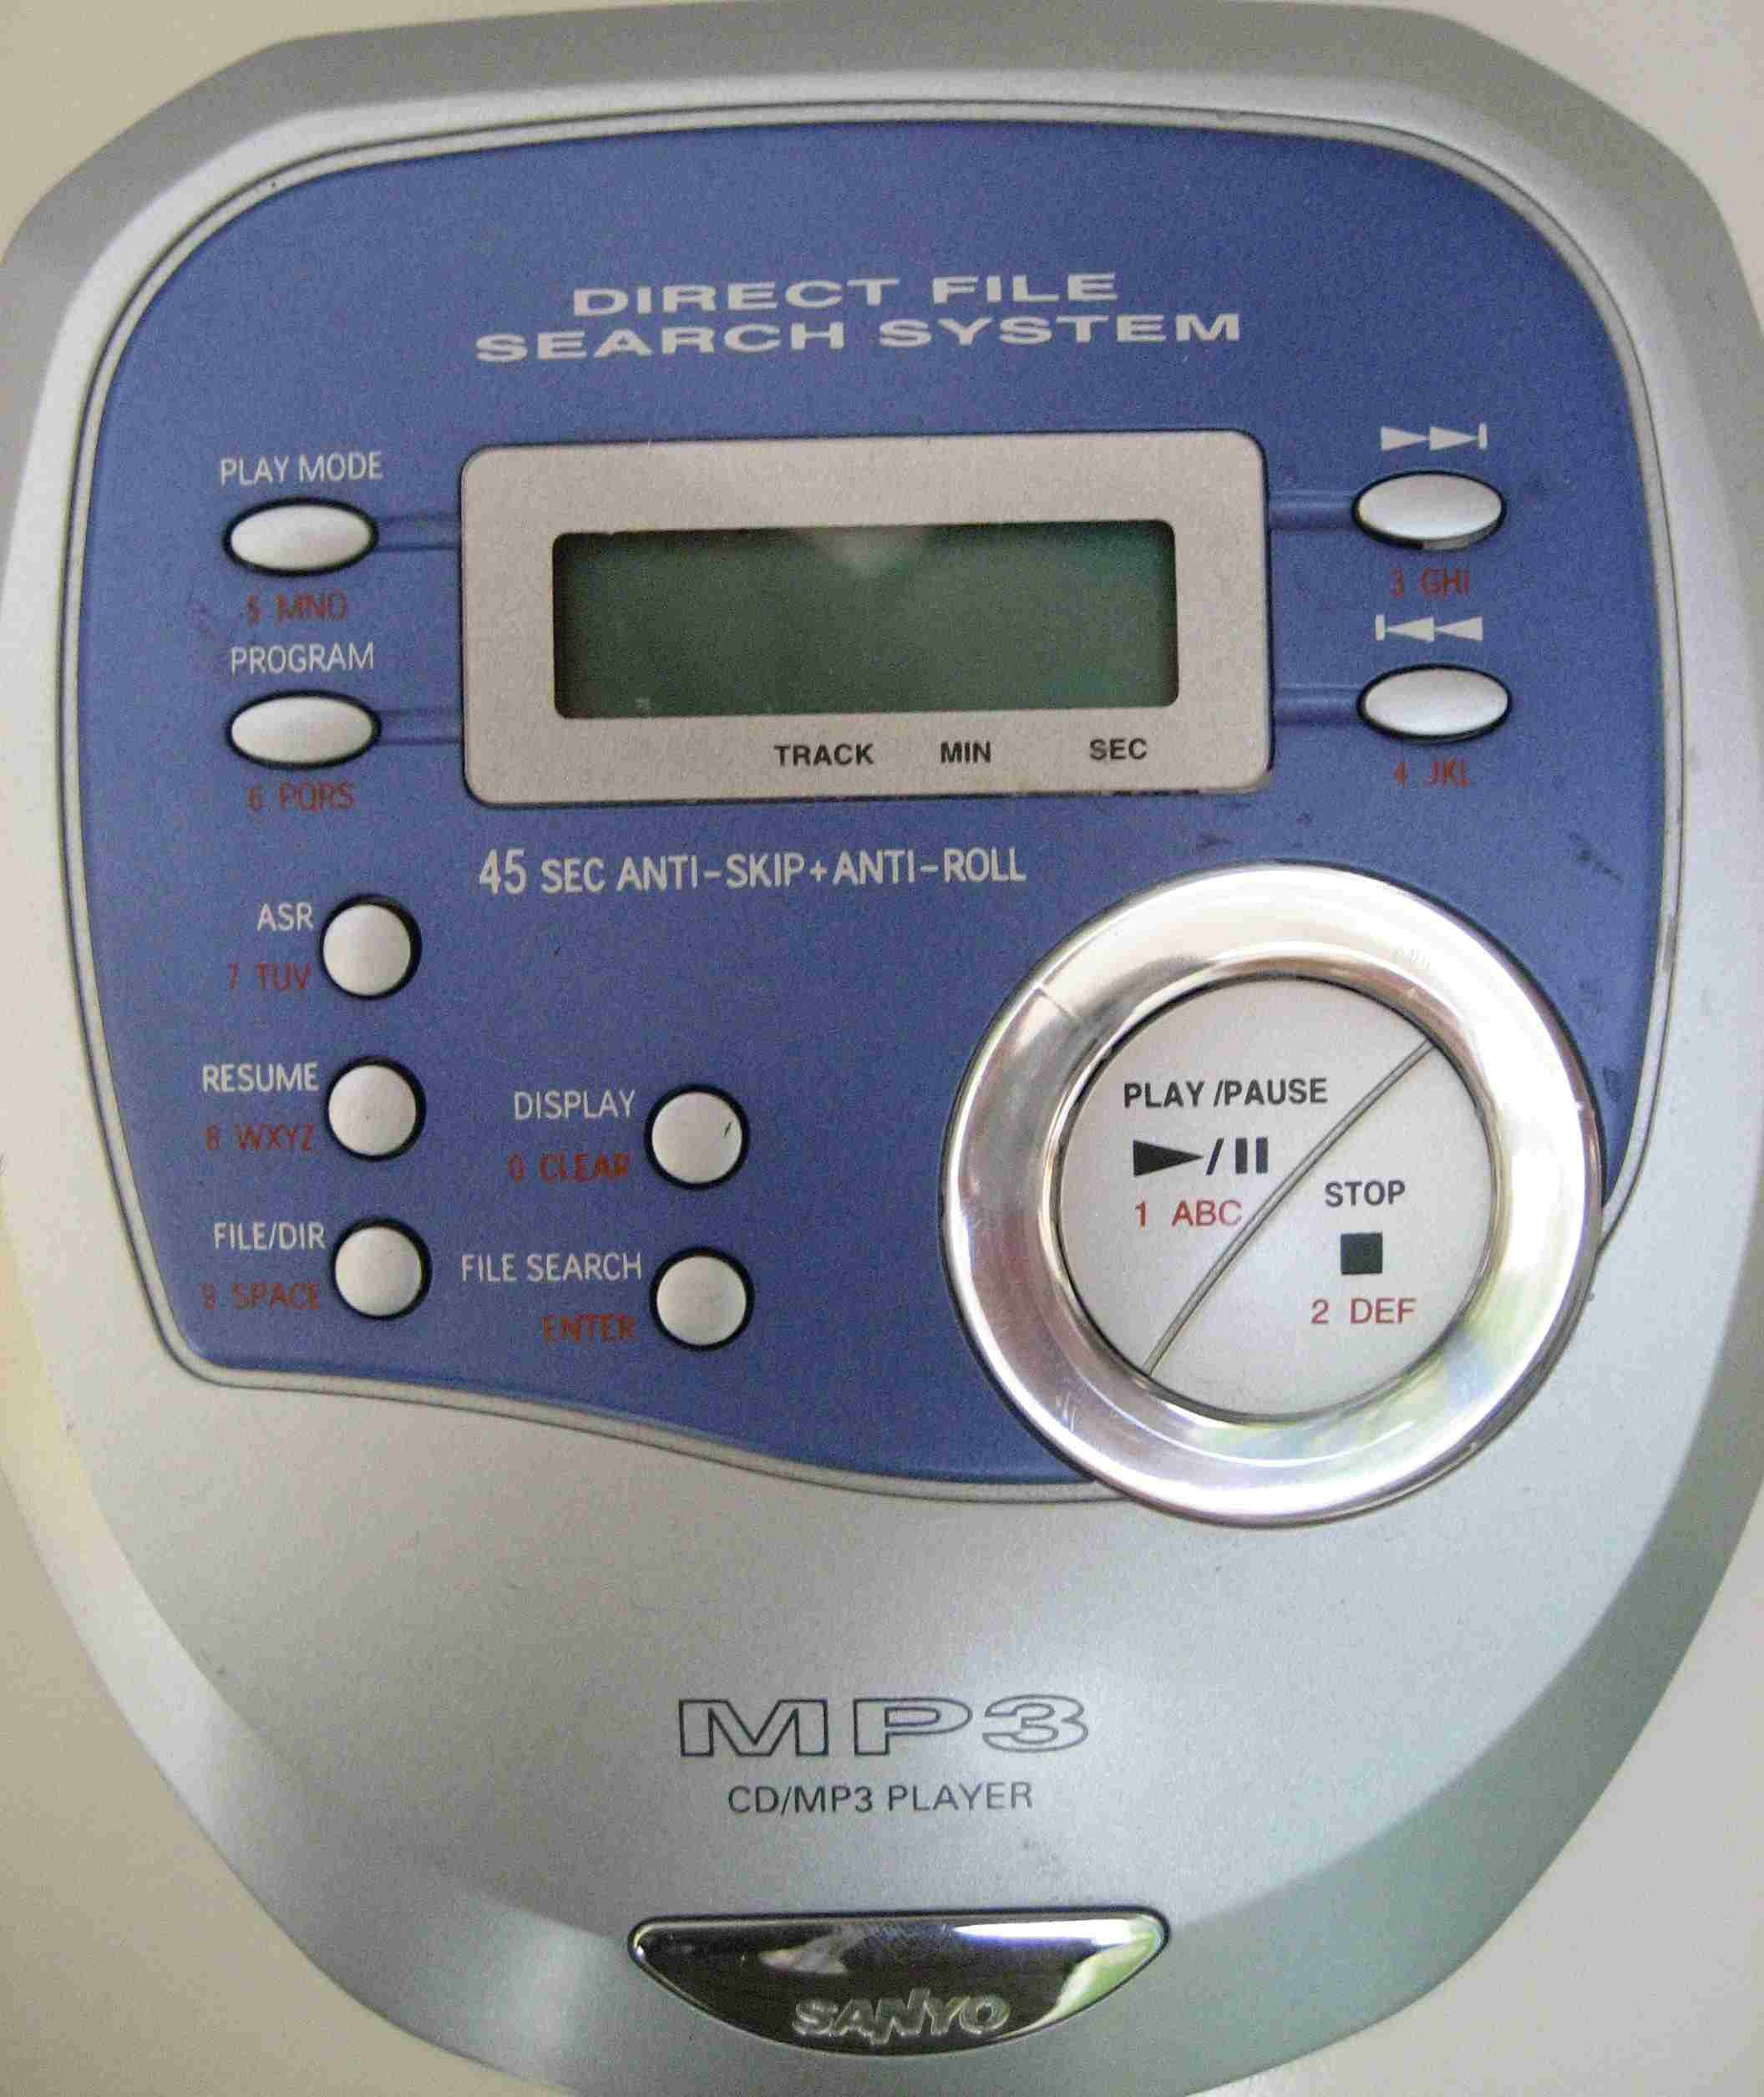
\includegraphics[width=.75\columnwidth]{Images/sanyo-photo.jpg}}
  \caption{Corpus 1: usability issues with an MP3-CD player device.}
  \label{tab:sanyo}
\end{figure}

\paragraph{Corpus 2} The second corpus contains a much larger number of student answers and covers eight questions.  Segmentation of answers into issues addressed is not relevant in this context.  The answers are taken from a college-level physics class.

General statistics on the two corpuses are reported in Table~\ref{tab:corpus}.

\begin{table}
  \caption{Inter-judge agreements}
  \label{tab:kappa}
  \begin{center}
    \begin{tabular}{rr@{}lr@{}l}
      \toprule
      & \multicolumn{2}{c}{Corpus 1} & \multicolumn{2}{c}{Corpus 2}\\
      \midrule
      Number of non-relevant texts \\ found by Judge 1 & 11&$\,$ & 286 \\
      \midrule
      Number of non-relevant texts \\ found by Judge 2 & 10&$\,$ & 297 \\
      \midrule
      Inter-judge agreement (Kappa) & \multicolumn{1}{r@{}}{95}&\multicolumn{1}{@{}l}{.0$\,$\%} & 97&\multicolumn{1}{@{}l}{.0$\,$\%} \\
      \bottomrule
    \end{tabular}    
  \end{center}
\end{table}

\begin{table}
  \caption{Corpus statistics}
  \label{tab:corpus}
  \begin{center}
    \begin{tabular}{rr@{}lr@{}l}
      \toprule
      & \multicolumn{2}{c}{Corpus 1} & \multicolumn{2}{c}{Corpus 2}\\
      \midrule
      Questions & 1&$\,$ & 8 \\
      Answers & 71&$\,$ & 2054 \\
      Students & 90& & 367 \\
      Non-relevant answers ratio & \multicolumn{1}{r@{}}{12}&\multicolumn{1}{@{}l}{.7$\,$\%} & 13&\multicolumn{1}{@{}l}{.8$\,$\%} \\
      \bottomrule
    \end{tabular}    
  \end{center}
\end{table}

\newpage
%%%%%%%%%%%%%%%%%%%%%%%%%%%%%%%%%%%%%%%%%%%%%%%%%%%%%%%%%%%%%%%%%%%%%%%%%%%%%
\section{Results}

\begin{table}
  \caption{Answer filtering results}
  \label{tab:res}
  \begin{center}
    
    \begin{tabular}{lcc}
      \hline
      & \multicolumn{2}{c}{$F_1$ scores}\\
      \cline{2-3}
            {Method} & Corpus 1 & Corpus 2\\
            \hline
            Average Cosine & 0.842 & 0.839 \\
            3-words rule & 0.250 & 0.797 \\
            \hline
    \end{tabular}
  \end{center}
\end{table}

Figure~\ref{tab:hist1} shows the distribution of average cosines for relevant and non-relevant answers.  The non-relevant answers do have an average cosine that is generally close or equal to~0.  

\begin{figure}
%  \includegraphics[width=\columnwidth]{Images/dalite_mean_distance_10clusters.png}
  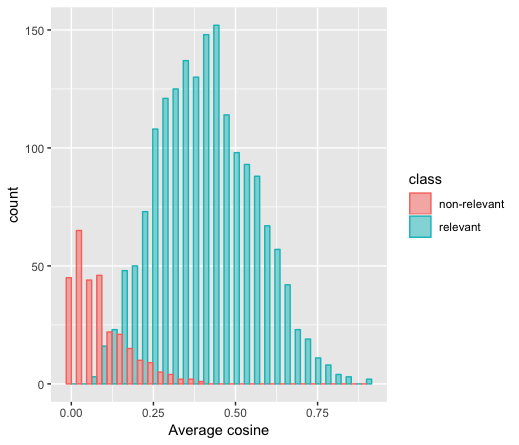
\includegraphics[width=\columnwidth]{Images/dalite_av_cosine_10clusters.png}
  \caption{Histogram of average cosines for relevant and non-relevant student answers.}
  \label{tab:hist1}
\end{figure}

The $F_1$ classification results of the experiments are reported in Table~\ref{tab:res}.  $F_1$ scores are calculated considering non-relevant answers as Positives, since the filtering aims to recall non-relevant as opposed to relevant answers (note that using relevant answers as Positives would give different scores).

The results are broken down by the methods described and compared with a simple baseline that is actually used in \dalite which consists in classifying answers that contain 3~words or less as irrelevant.

%% rule3 <- (sapply(strsplit(as.character(mydalite_data$Explication), " "), length))<4
%% F1_Score(!rule3,!(rater2=='x' | rater2=='xx'))



%%%%%%%%%%%%%%%%%%%%%%%%%%%%%%%%%%%%%%%%%%%%%%%%%%%%%%%%%%%%%%%%%%%%%%%%%%%%%
\section{Conclusion}

We propose a simple-to-implement, unsupervised approach to filter out undesired short and open student answers.  Undesired answers typically occur in student response systems such as peer learning environments, for eg.~\dalite, or in classroom app., for eg.~Socrative.  The approach is intended to be effective in a context where some answers are collected, but they are not labeled and no correct answer is provided either.  Moreover, the approach is intentionally tested with a small dataset because this is also often to be expected in practice.  It is compared with a trivial rule based on the number of words that, while parsimonious and effective, misses some undesired answers.

Results show that the approach improves on the simple rule, in particular for Corpus~1 which corresponds to the Socrative context and where the rule performs poorly.  A smaller improvement is found for the peer learning environment of Corpus~2.  Moreover, the $F_1$ score shows that not all irrelevant answers are filtered.

Nevertheless, the simplicity of the approach makes it an attractive means to address the undesired answer filtering issue in practice.
\vfill
\bibliographystyle{plain}
\bibliography{ref.bib}
\end{document}
